\ifx\PREAMBLE\undefined
\documentclass{report}
\usepackage[format = hang, font = bf]{caption}
\usepackage{graphicx}
\usepackage{array}
\usepackage{amsmath}
\usepackage{mathtools}
\usepackage{boxedminipage}
\usepackage{listings}
\usepackage{makecell}%diagonal line in table
\usepackage{float}%allowing forceful figure[H]
\usepackage{xcolor}
\usepackage{amsfonts}%allowing \mathbb{R}
\usepackage{alltt}
\usepackage{algorithmicx}
\usepackage[chapter]{algorithm} 
%chapter option ensures that algorithms are numbered within each chapter rather than in the whole article
\usepackage[noend]{algpseudocode} %If end if, end procdeure, etc is expected to appear, remove the noend option
\usepackage{xspace}
\usepackage{color}
\usepackage{url}
\def\UrlBreaks{\do\A\do\B\do\C\do\D\do\E\do\F\do\G\do\H\do\I\do\J\do\K\do\L\do\M\do\N\do\O\do\P\do\Q\do\R\do\S\do\T\do\U\do\V\do\W\do\X\do\Y\do\Z\do\[\do\\\do\]\do\^\do\_\do\`\do\a\do\b\do\c\do\d\do\e\do\f\do\g\do\h\do\i\do\j\do\k\do\l\do\m\do\n\do\o\do\p\do\q\do\r\do\s\do\t\do\u\do\v\do\w\do\x\do\y\do\z\do\0\do\1\do\2\do\3\do\4\do\5\do\6\do\7\do\8\do\9\do\.\do\@\do\\\do\/\do\!\do\_\do\|\do\;\do\>\do\]\do\)\do\,\do\?\do\'\do+\do\=\do\#\do\-}
\usepackage[breaklinks = true]{hyperref}
\lstset{language = c++, breaklines = true, tabsize = 2, numbers = left, extendedchars = false, basicstyle = {\ttfamily \footnotesize}, keywordstyle=\color{blue!70}, commentstyle=\color{red!70}, frame=shadowbox, rulesepcolor=\color{red!20!green!20!blue!20}, numberstyle={\color[RGB]{0,192,192}}}
\mathchardef\myhyphen="2D
% switch-case environment definitions
\algblock{switch}{endswitch} 
\algblock{case}{endcase}
%\algrenewtext{endswitch}{\textbf{end switch}} %If end switch is expected to appear, uncomment this line.
\algtext*{endswitch} % Make end switch disappear
\algtext*{endcase}
\begin{document}
\fi
\chapter{Runtime organization}
Up to now we have completed the front-end phase of the compiler: lexical analysis, parsing and semantic analysis. These three phases intend to enforce the language definitions. If no errors were generated during the front-end phases, the program proves to be valid in the language, and we are ready to proceed to the backend phases: optimization and code generation. However, before we can talk about the backend phases, we need to talk about runtime organization, which is essential to help us understand what we are trying to generate.

The main topics of this section include run-time resources management, correspondence static(compile-time) and dynamic (run-time)structures, and storage organization.

Exectution of a program is initially under the control of the operating system. When a program is invoked, the OS allocates space for the program, the code is loaded into part of the space, and the OS jumps to the entry point of the program, i.e. the ``main'' function. 

The memory space allocated for a program is not necessarily contiguous. Besides the part of space storing the code, the rest of the space stores data. The compiler is responsible not only for generating the code, but also for orchestrating the data area.
\section{Activations} 
We have two goals in code generation: the correctness of the code in the sense that it correctly implements the program intended by the programmer, and the speed of the program. Complications in code generation originates from the need to solve the two problems simutaneously. Over history, an elaborate framework has been developped to ensure that the two goals can be achieved together. Activation is the first topic in our discussion of the framework.

We will assume that the programming languages for which we are trying to generate code satisfy:
\begin{enumerate}
\item Execution is sequential. Control moves from one point in a program to another in a well defined order. This assumption is violated if a language supports concurrency. 
\item When a procedure is called, control always returns to the point immediately after the call. This assumption is violated if the language supports advanced control mechanism such as exceptions and call/cc.
\end{enumerate} 

An invocation of procedure P is called an \textbf{activation} of procedure P. The \textbf{lifetime} of an activation of P is all the steps to execute P, including all steps in procedures called by P. Similarly, we can define the \textbf{lifetime} of a variable x as the portion of execution in which x is defined. Note that lifetime is a dynamic/runtime concept, while scope is a static concept. 

From the definitions and our assumptions, it is clear that when procedure P calls procedure Q, Q must return before P returns. Thus lifetimes of procedure activations are properly nested, which makes them suitable to be depicted as a tree, i.e. the activation tree. The activation tree depends on runtime behavior, and can be different for different inputs. Since activations are nested, we can use a stack to track currently active procedures. The procedure stack comes after the part to store code in the memory. It grows when new procedure is called, and shrinks when the current procedure returns.

The information needed to manage one procedure is called an \textbf{activation record (AR)}, or a \textbf{frame}. Activation record keeps track of the information needed to properly execute a procedure. If procedure F calls G, the G's activation record contains a mix of information about F and G. In this case, F is suspended until G completes, at which point F resumes. G's AR contains information needed to complete the execution of G, and to resume execution of F. Condiser the following Cool procedure:
\begin{lstlisting}
Class Main {
	g():Int { 1 };
	f(x:Int):Int { if x=0 then g() else f(x-1) fi};
	main():Int { f(3) };
};
\end{lstlisting}

Main has no argument or local variables, and its result is never used. Thus its AR is not interesting. We will focus on the AR of f. The AR of f contains
\begin{itemize}
\item result of f (return value)
\item argument
\item control link (a pointer to the previous activation, i.e. the caller)
\item return address (memory address of the instruction to jump to after f completes, i.e. where execution resumes after a procedure call finishes)
\end{itemize}

This is just one of many possible AR designs. It would also work for C, Pascal, FORTRAN, etc. The advantage of placing the return value at the 1st position in a frame is that the caller can find it at a fixed offset from its own frame. An AR design is better as long as it improves execution speed or simplifies code generation. In practice, compilers hold as many frames in registers as possible, especially results and arguments of procedures.

The compiler must determine \textbf{at compile time} the layout of activation records and generate code that correctly accesses locations in the activation records. Thus, the AR layout and the code generator must be designed together.
\section{Globals and heap}
All references to a global variable point to the same object, thus they cannot be be stored in an activation record which is deallocated after an activation is completed. Globals are assigned a fixed address once, and we call these variables ``statically allocated'' because they are allocated during compile time. Depending on the language, there may be other statically allocated values.

Besides globals, a value that outlives the procedure that creates it cannot be kept in the AR either. For example, for the method \texttt{foo() \{new Bar\}}, the Bar value must survive the deallocation of foo's AR. Languages with with dynamically allocated data use a heap to store dynamic data. 

Now we can summarize different kinds of data that a language implementation has to deal with. 
\begin{itemize}
\item The code area contains object code. For many languages it is of fixed size and read-only.
\item The static area contains data with fixed addresses, e.g. globals. This area is of fixed size, and can be read-only or writable.
\item The stack contains an AR for each currently active procedure. Each AR is usually of fixed size, and contains the locals of the procedure.
\item Heap contains all other data. In C, heap is managed by \texttt{malloc} and \texttt{free}, while in JAVA there is \texttt{new} for allocation and garbage collection mechanism takes care of reclaimation of heap space no longer to be used.
\end{itemize}
Both stack and heap grows. We should make sure that they do not grow into each other. A simple solution is to let them start at opposite ends of the memory and grow towards each other. We end up with the partition of the memory shown in Figure \ref{mempart}. 
\begin{figure}[ht]
\centering
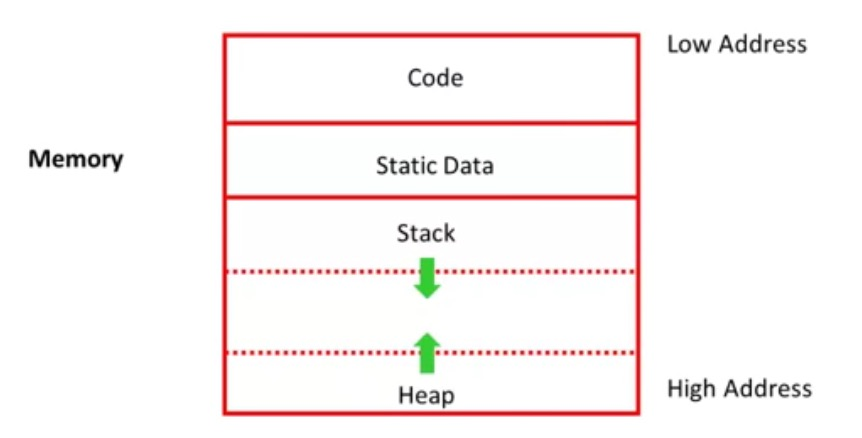
\includegraphics[width = 0.8\textwidth]{memory.jpg}
\caption{Partition of memory}\label{mempart}
\end{figure}
\section{Alignment}
Alignment is a very low-level but yet very important machine architecture detail for programmers trying to implement a compiler. Most modern machines are 32-bit or 64-bit, i.e. there are 4 or 8 bytes in a word. Machines are either byte or word addressable. A piece of data is said to be aligned if it begins at a word boundary. Most machines have some sort of alignment restrictions or performance penalties for poor alignment. 

\ifx\PREAMBLE\undefined
\end{document}
\fi